\subsection{Why Off-Center Feeding for a Dipole?}

\begin{tcolorbox}[colback=gray!10, colframe=black, title=E9C05] What is the purpose of feeding an off-center-fed dipole (OCFD) between the center and one end instead of at the midpoint?
\begin{enumerate}[label=\Alph*.]
    \item \textbf{To create a similar feed point impedance on multiple bands}
    \item To suppress off-center lobes at higher frequencies
    \item To resonate the antenna across a wider range of frequencies
    \item To reduce common-mode current coupling on the feed line shield
\end{enumerate} \end{tcolorbox}

In order to understand the purpose of feeding an Off-Center-Fed Dipole (OCFD) antenna between the center and one end, it is essential to familiarize ourselves with certain related concepts in antenna theory and feed point impedance. An OCFD antenna is designed to operate efficiently across multiple frequency bands, which means that its feed point needs to be strategically positioned to achieve this.

When an OCFD is fed at the midpoint, it primarily resonates at a single frequency, which limits its usability in multi-band applications. By moving the feed point closer to one end, we create an asymmetrical antenna where the impedance seen at the feed point changes. This variation in impedance allows the antenna to match closer to the feed line impedance across a broader frequency range, thus facilitating multi-band operation due to the different resonant frequencies that can be effectively utilized.

Let's analyze the choices presented:
- \textbf{Choice A:} is the correct answer, as it directly addresses the creation of a similar feed point impedance that allows for multi-band usage.
- \textbf{Choice B:} relates to antenna radiation patterns but doesn't specifically address the impedance aspect or the multi-band functionality.
- \textbf{Choice C:} describes a general property of antennas but doesn't elaborate on the specific feeding technique's advantages.
- \textbf{Choice D:} touches on common-mode currents, which is a separate issue of antenna design not directly related to the operational advantages gained through off-center feeding.

To further illustrate the concept, we can represent the feed point of the OCFD antenna with a simple diagram created using the TikZ package:

\begin{center}
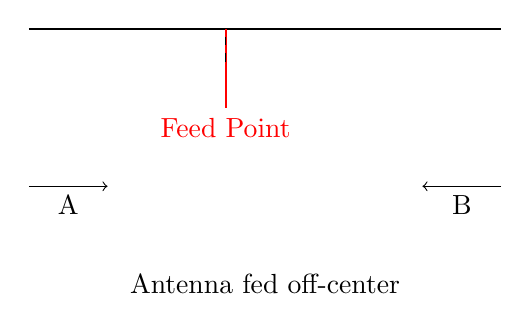
\begin{tikzpicture}
    \draw[thick] (0,0) -- (6,0); % The antenna
    \draw[red, thick] (2.5,0) -- (2.5,-1) node[below] {Feed Point}; % The feed point
    \draw[dashed] (2.5,-0.1) -- (2.5,-0.5);
    \draw[->] (0,-2) -- (1,-2) node[midway, below] {A}; % End of the dipole
    \draw[->] (6,-2) -- (5,-2) node[midway, below] {B}; % Other end of the dipole
    \draw (3,-3) node[below]{Antenna fed off-center};
\end{tikzpicture}
\end{center}

In summary, the strategic choice of the feed point location in an OCFD antenna design not only influences the impedance characteristics but also enhances its capacity for resonating across diverse frequency bands, which is a significant advantage for amateur radio operators and other practical applications in radio communications.
